\documentclass{report}

\usepackage[left=3cm,right=3cm,top=1cm,bottom=2cm]{geometry}
\usepackage{polski}
\usepackage[utf8]{inputenc}
\usepackage{graphicx}

\title{%
	System pisania testów na platformie Android \\
	\large Raport inżynierski}

\author{
	Filip Malinowski\\
	\texttt{filip.malinowski@student.pwr.edu.pl}
	\and
	pod przewodnictwem Promotora dr Witolda Paluszyńskiego\\
	\texttt{witold.paluszynski@pwr.edu.pl}
}
\date{}

\begin{document}

%\maketitle

	\chapter{Plan pracy}

	Tematem pracy jest stworzenie systemu na platformę Android umożliwiającego pisanie testów na wykładach akademickich i zautomatyzowane przetworzenie wyników testów. W skład systemu planowo mają wejść: aplikacja na system Android oraz aplikacja serwerowa, z którą aplikacja połączy się wysyłając wybrane przez użytkownika odpowiedzi.\\
	
	Na rynku istnieją już aplikacje częściowo odpowiadające tematowi pracy inżynierskiej. Ich funkcjonalność spełnia pewne aspekty jakimi są: wybór odpowiedzi, przesyłanie odpowiedzi do serwera oraz pobieranie treści z serwera na aplikację. Najlepszym przykładem jest aplikacja nazywająca się Quizowanie \footnote{https://play.google.com/store/apps/details?id=se.feomedia.quizkampen.pl.lite}. Aplikacja ta pozwala na pobieranie i wyświetlenie pytań z serwera, wyświetlenie możliwych odpowiedzi jako przycisków dla użytkownika oraz wysłanie odpowiedzi do serwera i zweryfikowanie ich. Jej kod źródłowy jest jednak zamknięty co sprawia, że jest nieprzydatny przy tworzeniu systemu będącego tematem tej pracy.
	
	Inne aplikacje, które można wymienić to English Grammar Test\footnote{https://play.google.com/store/apps/details?id=english.grammar.test.app} lub też sameQuizy\footnote{https://play.google.com/store/apps/details?id=pl.filing.samequizy}. Ich wartość ogranicza się jednak do rozwiązań dotyczących wyglądu interfejsu aplikacji. Nie ma możliwości w legalny sposób uzyskać kodu źródłowego lub opisów rozwiązań w tych aplikacjach z racji ich komercyjnego zastosowania.
	\\
	W przypadku aplikacji serwerowej jest wiele możliwych technologii, które można zastosować przy jej tworzeniu. Pierwszym etapem był wybór protokołu komunikacyjnego jaki zostanie użyty między aplikacją androidową, a serwerem. Możliwe protokoły to np. TCP, UDP, POP, SMTP, HTTP czy FTP. Wybrany został protokół HTTP z powodu tego, że sieć WiFi na Politechnice Wrocławskiej ma odblokowaną komunikację na portach 80 oraz 8080 oraz prawdopodobnie na tych wymienionych portach sprawdzane są też użyte protokoły i ich zgodność z HTTP. Innego rodzaju protokół wykluczyłby użycie systemu w połączeniu z politechniczną siecią WiFi co znacząco obniżyłoby jego zastosowanie.
	
	Kolejnym etapem był wybór odpowiedniego odpowiedniego serwera web do obsługi zapytań przesłanych z aplikacji mobilnej. Możliwe aplikacje serwerowe jakie można wykorzystać to: Apache, nginx, lighttpd, OpenLiteSpeed. Początkowe wersje aplikacji mobilnej komunikują się z serwerem Apache\footnote{https://httpd.apache.org/} jednak docelowo ma zostać do tego użyty nginx\footnote{https://www.nginx.com/}. Z racji tego, że większość serwerów obsługuje FastCGI pozwalających na napisanie programu obsługującego zapytania w wielu popularnych językach, to przy wyborze serwera kierowano się jego wydajnością obsługi zapytań przychodzących. Wykorzystano tutaj Linux Web Server Performance Benchmark\footnote{https://www.rootusers.com/linux-web-server-performance-benchmark-2016-results/} z 2016.
	
	
	\begin{center}
		\begin{figure}[ht]
			\centering
			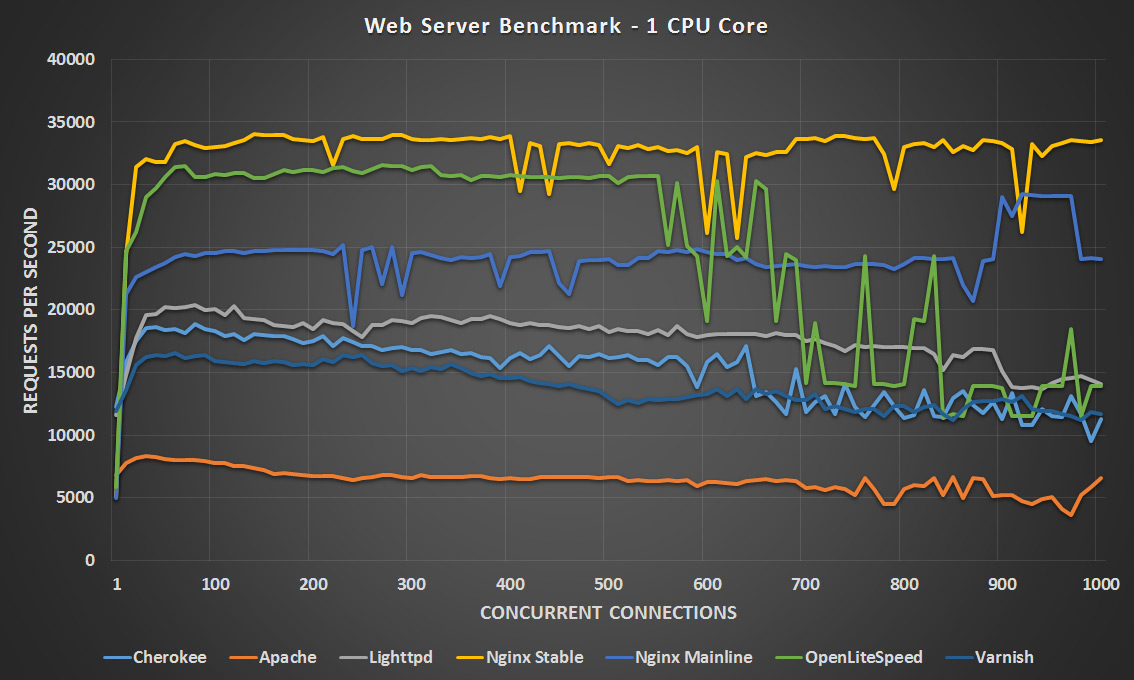
\includegraphics[scale=0.3]{web-server-performance-benchmark-1-cpu-core-1.jpg}
			\caption{Wykres przedstawiający ilość obsługiwanych zapytań przy danej ilości otwartych połączeń z Linux Web Server Performance Benchmark}
		\end{figure}
	\end{center}
	
	
	Należało też wybrać środowisko w jakim aplikacja mobilna powinna powstać. W tym przypadku do wyboru jest Android Studio\footnote{https://developer.android.com/studio/index.html} oraz Qt\footnote{https://www.qt.io/}. Oba środowiska oferują duże wsparcie ze strony społeczności programistycznej oraz szeroki zestaw narzędzi. Oba pozwalają na tworzenie interfejsu użytkownika w XML oraz udostępniają klasy obiektów przydatne do wizualizowania i przetwarzania danych. Wybrany został jednak Android Studio z racji jego największej popularności oraz najszerszej gamy narzędzi wchodzących w skład tego środowiska. Pozwala na dołączanie bibliotek z repozytoriów Git lub też bibliotek za pomocą wbudowanego narzędzia Maven\footnote{https://maven.apache.org/}, bieżące sprawdzanie kompatybilności użytych bibliotek z wersjami systemu Android na które aplikacja powstaje oraz tworzenie maszyn wirtualnych do testowania napisanych aplikacji.
	\\
	Zważywszy na powyżej przedstawione informacje system do rozwiązywania testów musi być napisany od podstaw. Nie znaleziono przykładów otwartych systemów na tyle użytecznych, żeby można było użyć ich przy tworzeniu systemu. Systemy takie jak Quizowanie mają zamknięty kod i można się nimi sugerować jedynie w kwestii tworzenia interfejsu użytkownika.
	
	W trakcie pracy nad systemem do rozwiązywania testów wymagania co do tego systemu zostały doprecyzowane. Aplikacja mobilna musi być przyjazna dla użytkownika i intuicyjna. Użytkownik dalej ma możliwość pisania testów na papierze dlatego forma elektroniczna musi być wystarczająco zachęcająca. Ponadto musi też być niezawodna. Nie powinna tracić przetwarzanych w niej istotnych informacji lub wyłączać się w trakcie rozpoczęcia pisania testu. Aplikacja musi się też w niezawodny sposób łączyć z serwerem w celu przesłania odpowiedzi użytkownika lub też pozwolić na ponowne ich wysłanie po utracie połączenia. Kopie zapasowe testów muszą też być zapisywane w pamięci wewnętrznej telefonu, a ich zawartość zaszyfrowana chroniąc wrażliwe dane przed ingerencją osób nieupoważnionych. Aplikacja powinna też być weryfikowalna przez serwer, żeby nie dopuścić do wysyłania odpowiedzi aplikacji zmodyfikowanych przez osoby trzecie. Musi też informować użytkownika odpowiednimi komunikatami wyświetlanymi na ekranie o zaistniałych problemach na każdym etapie użytkowania, żeby użytkownik wiedział w jaki sposób reagować na nieprzewidziane sytuacje.
	
	Aplikacja serwerowa musi być w stanie obsługiwać sprawnie wysoki ruch, w którym przybywa średnio 10 zapytań na sekundę dochodzących nawet do 100 na sekundę przy 100 osobowej grupie użytkowników piszących na aplikacji test. Docelowo powinna jednak być w stanie obsłużyć nawet 300-400 użytkowników, żeby można było ją zastosować w każdej możliwej grupie studentów na Politechnice Wrocławskiej. Serwer musi też być w stanie weryfikować łączące się aplikacje, tak aby nie przesyłać wrażliwych informacji do nieupoważnionych osób. Jego struktura musi być możliwie prosta, żeby przyszłe modyfikacje były mało uciążliwe dla użytkownika całego systemu.
	\\
	
	\chapter{Stopień zaawansowaia prac}
	
	Aplikacja mobilna przechowuje dane użytkownika takie jak: Imię, Nazwisko, numer indeksu oraz nazwa przedmiotu na którym wykonywany jest test. Umożliwia też zmianę adresu serwera, na który przysyłane są odpowiedzi z testu. Dane te zmienia się w ustawieniach aplikacji. W menu głównym pozwala na wprowadzenie rzędu i miejsca, na którym student siedzi podczas testu, wektora wag służącego do obliczania grupy oraz ID testu jaki jest przeprowadzany. Zostało też zaimplementowane udogodnienie dla studenta w postaci skanera kodów QR umożliwiającego zautomatyzowane wczytanie wektora wag, ID testu i wyliczenie grupy studenta. Do skanowania kodów QR została wykorzystana biblioteka zxing\footnote{https://github.com/zxing/zxing}. Po przejściu do testu wyświetlany jest ekran konfiguracyjny aplikacji gdzie student jest informowany o operacjach przeprowadzanych przed rozpoczęciem testu. Na obecnym etapie prac aplikacja sprawdza osiągalność serwera, do którego wysyła odpowiedzi oraz pobiera plik konfiguracyjny zawierający takie dane jak minimalna i maksymalna wersja aplikacji dopuszczona do testu oraz klucz szyfrowania danych w plikach testu przechowywanych na telefonie użytkownika. Po przejściu do testu wyświetlana jest zakładka pytania, a na niej: nr grupy w jakiej student jest, nr pytania, przyciski do wysłania odpowiedzi "tak", "nie", "nie wiem"; przyciski do dodania pytania i do podsumowania testu oraz unikalny identyfikator sesji wygenerowany dla aktualnej sesji testowej otwartej na telefonie. Dodanie pytania wymusza przejście do następnego pytania a UI użytkownika pozwala na przesuwanie ekranu w celu dostania się do innych pytań. Podsumowanie testu wyświetla ilość poprawnie przesłanych odpowiedzi "tak", "nie" oraz "nie wiem" do serwera, oraz ilość odpowiedzi zapisanych w pliku testowym. W razie różnicy w odpowiedziach przesłanych do serwera a zapisanych w pliku aplikacja wyświetla odpowiednie ostrzeżenie sugerujące użytkownikowi powrót do testu i ponowne przesłanie odpowiedzi. Na ekranie podsumowania wyświetlany jest przycisk pozwalający powrót do testu oraz przycisk kończący test powodujący powrót do menu głównego aplikacji.
	
	Obecnie serwerem do obsługi zapytań sieciowych jest Apache. Do przetwarzania danych wykorzystano skrypt napisany w języku AWK. Skanuje on logi serwera Apache w poszukiwaniu zarejestrowanych zapytań przysłanych z aplikacji mobilnych i umożliwia zapisanie ich w formacie użytecznym dla użytkownika całego systemu.
	
	Stworzony został też deszyfrator plików przechowywanych na telefonach studentów pozwalający na odzyskanie odpowiedzi studenta w razie problemów z połączeniem z serwerem gdy nie wszystkie odpowiedzi do niego dotarły.
	
\end{document}